\chapter[Include and looping: Data reuse]{Include and looping: Data reuse}
\label{subst}

Often in constructing a model it is possible to replicate one part to produce
a new part of the mesh.  \textsl{FEAP} provides several options to facilitate
such reuse.  The basic method is to place the part of the problem to be
reused in a separate file, called an include file, and to input the data by
adding a statement \texttt{INCLude filename} where the data is to be 
inserted.  This feature is described in the next section.  A second option
is to mark the data using a \texttt{SAVE} command and to \texttt{READ} the
data where it is again needed.  This is described in Section \ref{save}.
Finally, it is possible to reread the data parts several times using a
\texttt{LOOP-NEXT} option as described in Section \ref{mloop}.

\section{Include commands in mesh input}
\label{include}
\index{Mesh command!Include files}
\index{Mesh command!INCLude}
\index{Include files}

Any set of data input records may be placed in a separate file and read using
the \texttt{INCLude} command.  The form for an include is a single record
\begin{verbatim}
       INCLude filename
\end{verbatim}
where \texttt{filename} is the name of the file containing the input data items.
This command may be used at any time and include files may call other
include files (to a maximum level of 9).  Thus, if the nodal coordinates
are created by another program and written to a file named \texttt{Blockxy}
{\footnote{Upper and lower case letters are different in UNIX or LINUX 
environment but the same in a Windows one}},
they may be input as \textsl{FEAP} data using:
\begin{verbatim}
       COORdinates
       INCLude Blockxy
                          ! blank termination record
\end{verbatim}
The information in each file must always be in the format required by
\textsl{FEAP}.
If another format is written, then it is necessary to either translate the
data to the correct form or to write and link a user routine which can
input the data.
The creation of user routines is discussed in the \textsl{FEAP Programmers
Manual}\scite{feapp}.

\section{READ and SAVE commands in mesh input}
\index{Mesh command!READ}
\index{Mesh command!SAVE}
\label{save}

A group of mesh input statements also may be retained for future use by
placing them between the statements
\begin{verbatim}
       SAVE,filename
       .....
       .....
       SAVE,END
\end{verbatim}
{\tt filename} may be any 1 to 15 alphanumeric characters. Thus if
a {\tt SAVE MSH1} is used a new file named {\tt MSH1} will be
created to store the mesh commands to be saved.

For example, the following option may be used to generate nodal
forces with a variation in a load parameter.
\begin{verbatim}
       PARAmeter
         a= 5.
                       ! end with blank record
       SAVE,msh1       ! may also be SAVE mes1
       PARAmeter
         b= a/2
                       ! end with blank record
       FORCe
         31,0,b
         32,1,a
         34,0,a
         35,0,b
                       ! end with blank record
       SAVE,END
\end{verbatim}
A different loading state may then be specified by:
\begin{verbatim}
       PARAmeter
         a= -4.
                       ! terminator
       READ,msh1
\end{verbatim}
The value of $b$ will be recomputed using the new value of $a$
and the nodal forces will then be recomputed.  Many options are
possible using the features of parameters, expressions, INCLude, and SAVE
and READ commands.

\section{LOOP-NEXT to replicate mesh parts}
\label{mloop}
\index{Mesh command!LOOP}
\index{Mesh command!NEXT}
\index{Looping input}

Many models for problems analyzed by finite element methods have mesh parts
which are similar except for stretching and rotation transformations.
\textsl{FEAP} provides input capabilities to generate the model using
\texttt{LOOP}-\texttt{NEXT} commands.  The basic input structure is given
by the command sequence
\begin{verbatim}
       LOOP,n
         ...
       NEXT
\end{verbatim}
where $n$ defines the number of times to repeat the commands contained
within the loop.  The value of $n$ may be a constant or a parameter.
Any standard \textsl{FEAP} mesh commands may be used between the \texttt{LOOP}
and \texttt{NEXT} statements, however, it is easiest to use commands which do
not require explicit definitions for node or element numbers.

\begin{figure}[hb!]
\centerline {\hfil 
\includegraphics[height=2.2in]{figs/lp2blk} \hfil}
\caption{Two blocks using \texttt{LOOP-NEXT} commands \label{floop.0}}
\end{figure}
A simple example is the repetition of two blocks of identical elements
in which the material number is different.  Assume first that a file
named \texttt{Imblock} is constructed which contains the commands
\begin{verbatim}
       BLOCk
         CART n1 n2 0 0 ma
           1   0  0
           2   a  0
           3   a  b
           4   0  b

       PARAMeter
          ma = ma + 1

\end{verbatim}
Then a second file is given which defines the initial values of parameters
and the looping control.  This file is given by the statements shown in
Table \ref{tloop.1}
where we note the use of the loop using the \texttt{TRANsform} command. 
\begin{table}[ht!]
\begin{center}
\begin{verbatim}
       FEAP * * Two block problem
         0  0  0  2  2  4
       PARAmeters
         a  = 5
         b  = 4
         n1 = 6
         n2 = 3
         ma = 1
 
       LOOP,2
         INCLude Imblock
         TRANsform
           1 0 0
           0 1 0
           0 0 1
           a 0 0
       NEXT
       MATE 1
         SOLID
           ELAStic ISOTropic 1000 0.25

       MATE 2
         SOLID
           ELAStic ISOTropic 2000 0.25

       END
\end{verbatim}
\caption{\texttt{LOOP-NEXT} mesh construction \label{tloop.1}}
\end{center}
\end{table}
The above example produces the mesh shown in Fig. \ref{floop.0} and
is trivial (also not much is gained over a construction
using two block commands directly).

\begin{figure}[ht!]
\centerline {\hfil 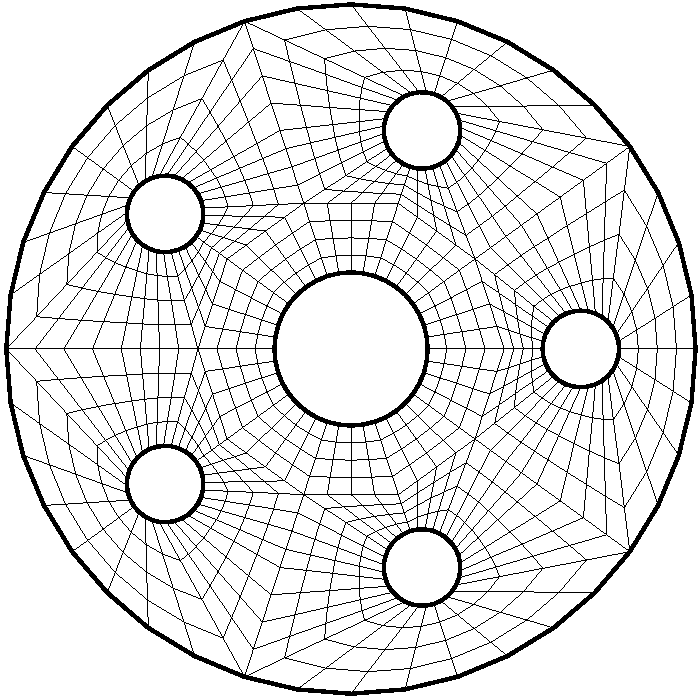
\includegraphics[height=3.5in]{figs/wheel5} \hfil}
\caption{Disk with holes \label{floop.1}}
\end{figure}
A more involved example is shown 
in Fig. \ref{floop.1} for a disk containing circular holes.  This
example was constructed using the commands shown in Table \ref{tloop.2}.
\begin{table}[ht!]
\begin{center}
\begin{verbatim}
       LOOP 5
         TRANSform
           cosd(th)  sind(th)    0
          -sind(th)  cosd(th)    0
               0         0       1
               0         0       0
         INCLude Iwseg
         TRANSform
           cosd(th)  sind(th)    0
           sind(th) -cosd(th)    0
               0         0       1
               0         0       0
         INCLude Iwseg
         PARAmeter
           th = th + 72

       NEXT
\end{verbatim}
\caption{\texttt{LOOP-NEXT} disk mesh construction \label{tloop.2}}
\end{center}
\end{table}
The file \texttt{Iwseg} contains the mesh for one part of the repeating
mesh as shown in Fig. \ref{floop.2}.
\begin{figure}[ht!]
\centerline {\hfil 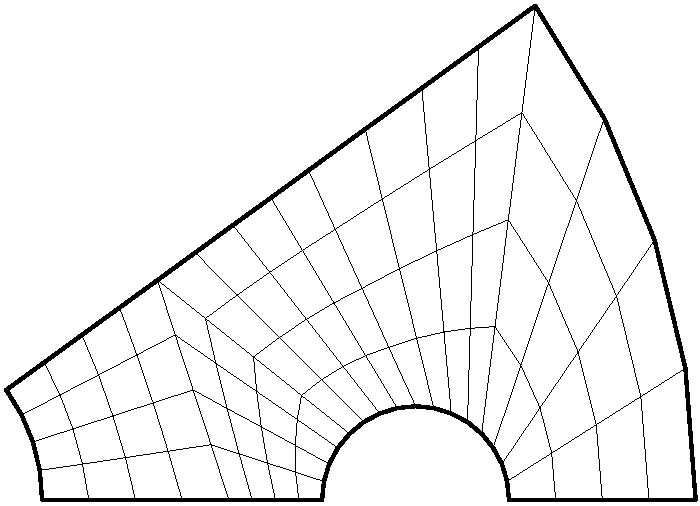
\includegraphics[height=2.0in]{figs/wheelsg} \hfil}
\caption{Mesh segment for disk with holes \label{floop.2}}
\end{figure}

Many more involved mesh constructs may be considered using the
\texttt{LOOP}-\texttt{NEXT} commands.  When using this option with blending
functions, however, \textit{do not} place \texttt{SNODe} or \texttt{SIDE}
commands within any looping instructions.  In this case a correct
structure is:
\begin{verbatim}
       SNODe
         1   ...
             etc.

       SIDE
         POLAr   ... (or other)
             etc.

       LOOP,n
         TRANsform coordinates
           ....

         BLENd
           .....
           etc.
       NEXT
\end{verbatim}
As a rule, any other commands which describes node or elements may
be placed within a \texttt{LOOP-NEXT} pair.

\section{Node and element numbers: \texttt{*NOD} and \texttt{*ELE}}
\label{stars}
\index{Mesh command!Setting node number}
\index{Mesh command!Setting element number}
\index{Mesh command!*ELEment}
\index{Mesh command!*NODe}

When using the include and loop options described above it is often necessary
to assign new node and element numbers to the input values.  It is
possible to set node numbers using parameters with constructs such as
\begin{verbatim}
       COORdinates
         n+1 1  0.0 0.0
         n+5 0 10.0 0.0
         ...
\end{verbatim}
and then reassign the value of the parameter \texttt{n}.   However, a more
expedient method is to use the \texttt{*NODe} and \texttt{*ELEment} option.

To use a \texttt{*NODe} option a command
\begin{verbatim}
       *NODe = 'expression'
\end{verbatim}
where \texttt{'expression'} can be any \textsl{FEAP} constant, parameter or
function expression.  The value obtained from the expression will then be
added to any nodal values appearing in an input.  For example an input of
an element statement as:
\begin{verbatim}
       ELEMent
          5 0 1 32 45
          ....
\end{verbatim}
would add the current value of the \texttt{*NODe} to the input values
\texttt{32} and \texttt{45} to produce new values of the nodes for this
element.

Use of a \texttt{*ELEment} option is given by a command
\begin{verbatim}
       *ELEment = 'expression'
\end{verbatim}
and any input of an element value would be incremented by the value of the
expression.

It is not necessary to use the \texttt{*NODe} and/or \texttt{*ELEment}
commands with \texttt{BLOCk} or \texttt{BLENd} inputs.

The default value for \texttt{*NODe} and \texttt{*ELEment} is zero.
